\section{Stripmap equivalent CSLC}
\label{sec:stripeq}

\subsection{Evaluation criteria}
\label{sec:stripeq_criteria}

The Stripmap-equivalent \acs{stripeq} \acs{cslc} image is a full-resolution \acs{sar} image (matching the resolution of the input) that combines multiple bursts from wide-area acquisition modes, such as Terrain Observation by Progressive Scans SAR (\acs{topsar}) or ScanSAR, to produce one seamless image with the spatial consistency and phase integrity of \acs{sm} mode.

Managing SAR acquisitions in burst mode is inherently more complex than conventional \acs{sm} acquisitions. The (\acs{stripeq}) product has been devised to hide this complexity from downstream processors, enabling burst-mode data to be ingested by existing Stripmap oriented processing chains without modification. Therefore, the \acs{stripeq} product must remain fully compatible with standard amplitude and phase-based workflows, including radiometric image generation, interferogram formation, and coherence estimation.

Burst-based acquisition modes impose an additional, azimuth-dependent phase modulation because the antenna beam is continuously steered during the synthetic aperture time. If left uncorrected, this modulation introduces phase discontinuities in the overlap regions between adjacent bursts, degrading interferometric coherence. Consequently, dedicated processing steps must be applied to ensure phase continuity and Doppler alignment before the bursts are coherently mosaicked. Therefore the chosen evaluation criteria for this product are indicators that measure (i) the phase continuity across former burst boundaries and (ii) the spatial homogeneity of coherence maps derived from co‑registered \acs{stripeq} image pairs. These metrics ensure that the final product meets the precision requirements for interferometric, change‑detection, and time‑series applications.

\subsection{Theoretical models}
\label{sec:stripeq_models}


Burst-mode acquisitions scanned in azimuth (\acs{topsar}, ScanSAR) introduce a deterministic, azimuth-dependent Doppler centroid $f_{DC}(\eta)$ due to the variation of the squint angle in the azimuth direction. This variation produces a pronounced phase modulation that can significantly degrade the quality of the resulting interferogram.

In ideal conditions—where master and slave images are perfectly co-registered in azimuth—the phase modulation cancels out during interferogram formation. However, in realistic scenarios, even a small residual co-registration error between the reference and slave images results in incomplete cancellation, leaving a residual phase ramp in each burst interferogram. The magnitude of this residual is directly related to the degree of misregistration. When such burst interferograms are mosaicked, phase discontinuities manifest at the burst overlap regions, as illustrated in Figure~\ref{fig:ESD_example}. This figure shows the phase mosaics obtained using the same master and two different slaves. The phase jumps are less visible in the left panel than in the right panel, due to the lower misregistration present in the left case compared to the right.

\begin{figure}[h!]
\centering
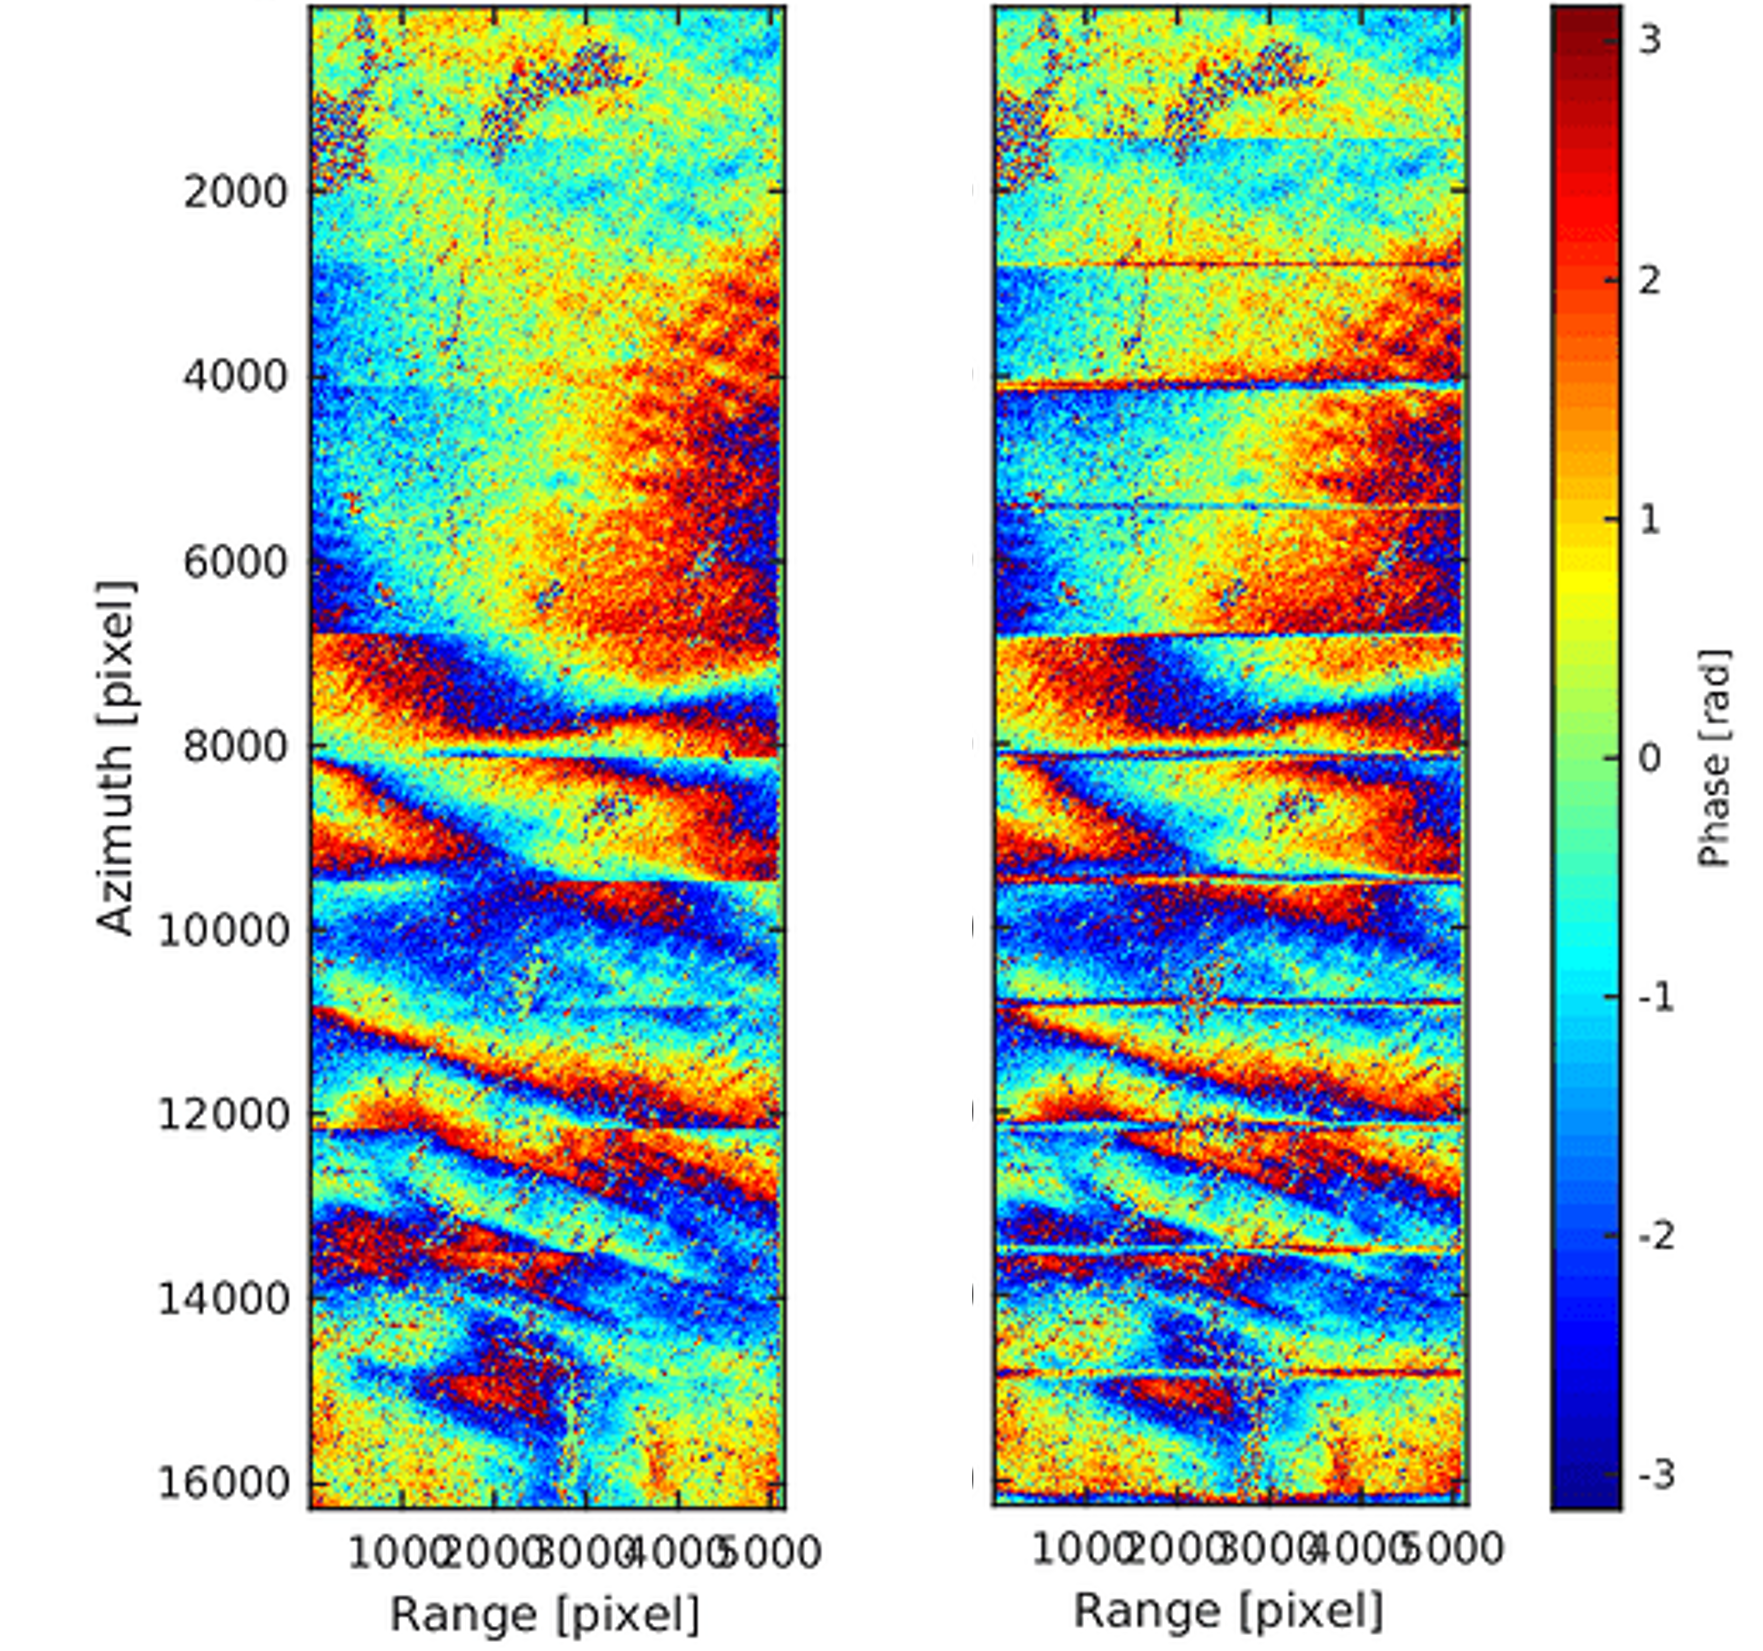
\includegraphics[width=0.9\textwidth]{Figures/strip_eq/ESD_example.png}
\caption{Interferometric phase mosaics derived from the same master image and two different slave acquisitions (\acs{s1} IW mode). The left panel exhibits smaller phase discontinuities across burst boundaries due to an higher accurate azimuth co-registration. In contrast, the right panel shows visible phase jumps resulting from increased residual misregistration, highlighting the critical need for sub-pixel accuracy in burst alignment for phase sensitive applications.}
\label{fig:ESD_example}
\end{figure}

More formally, using a small-angle approximation, a residual azimuth co-registration error of $\Delta t$ seconds introduces a phase ramp across the burst interferogram:

\begin{equation}
\Delta \phi_{az} = 2\pi \Delta f_{DC}\Delta t = \lambda \Delta \beta \Delta t
\label{eq:phase_jump}
\end{equation}

Here, $\Delta f_{DC}$ is the Doppler centroid variation, $\Delta \beta$ the corresponding change in squint angle, and $\Delta t$ the azimuth misregistration.

This relationship forms the basis for defining the accuracy requirements of azimuth co-registration to avoid phase jumps that could compromise the usability of \acs{stripeq} products for phase sensitive applications. For Sentinel-1, with a maximum $\Delta f_{DC}$ of approximately 5 kHz, limiting the phase ramp to 1/100 of a cycle (≈3.6°) requires a co-registration accuracy of about 0.001 pixels—equivalent to roughly 1.3 cm at the sensor's azimuth sampling rate.

Such stringent precision surpasses the capabilities of traditional methods like cross-correlation using small patches, where correlation peaks often provide only pixel level (or at most an accuracy of about 0.1 pixels) estimates. 

Considering the ROSE-L mission, the expected Doppler centroid variation is significantly lower than that of \acs{s1}. For \acs{rosel}, $\Delta f_{DC}$ is estimated to be approximately 1.4 kHz, resulting in a less stringent co-registration requirement in the azimuth direction. Nevertheless, if we still aim to limit the phase ramp to 1/100 of a cycle ($\approx 3.6°$), the required co-registration accuracy remains around 0.01 pixels-an order of magnitude more relaxed than in the \acs{s1} case, yet still beyond the capabilities of conventional co-registration methods based on standard cross-correlation.

Figure~\ref{fig:CRG_vs_FDC} illustrates the required co-registration accuracy (expressed in meters) as a function of $\Delta f_{DC}$, under different tolerances for allowable phase jumps between consecutive bursts. The two vertical dotted lines represent the \acs{s1} (red) and \acs{rosel} (yellow) configurations, based on the maximum $\Delta f_{DC}$ values anticipated for each SAR mission.

\begin{figure}[h!]
\centering
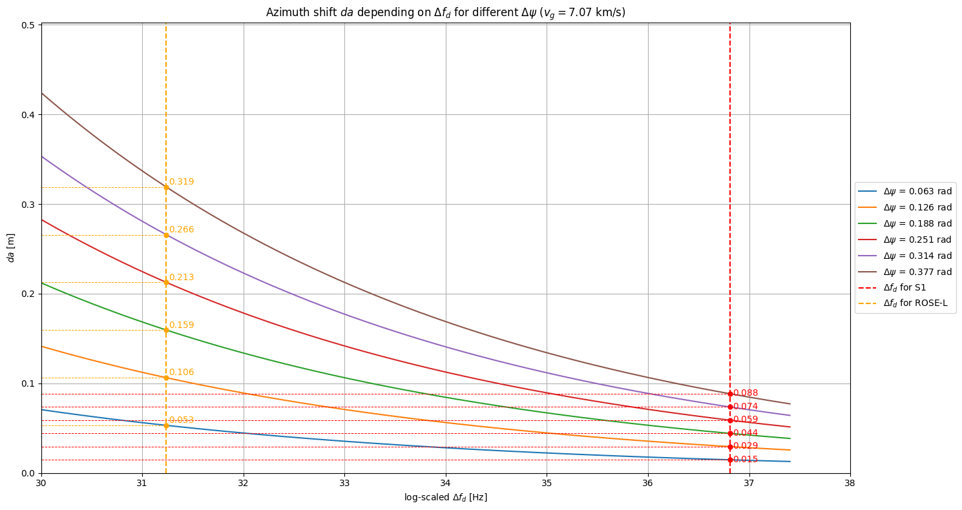
\includegraphics[width=0.9\textwidth]{Figures/strip_eq/CRG_accuracy_vs_fdc.png}
\caption{Required co-registration accuracy in meters as a function of Doppler centroid variation $\Delta f_{DC}$, under different thresholds of allowable phase jumps across burst boundaries. The red and yellow vertical lines correspond to \acs{s1} and \acs{rosel} mission parameters, respectively.}
\label{fig:CRG_vs_FDC}
\end{figure}

The previously discussed considerations highlight that to obtain a valid \acs{stripeq} \acs{ard} product, advanced techniques such as Spectral Diversity (SD) or Enhanced Spectral Diversity (ESD)—which analyse phase differences in burst overlap regions—must be employed.

The Spectral Diversity (SD) approach \citep{Scheiber2000} uses frequency shifts between azimuth looks, induced by the interferometric baseline, to estimate $\Delta t$ with sub-pixel accuracy by measuring phase differences in the azimuth sub-band cross-spectrum.

The Enhanced version of Spectral Diversity (\acs{esd}) \citep{Martínez2016} refines SD for \acs{topsar} mode. This method achieves empirical accuracies of approximately $10^{-4}$ pixels, comfortably within the Sentinel-1 requirement.

It must be highlighted that the requirement for the creation of a valid \acs{stripeq} \acs{ard} product also depends on the quality of the \acs{cslc} input data, from which consecutive bursts and subswaths are merged to create a Stripmap-like product. Once the previously described co-registration accuracy in the azimuth direction is met—by applying advanced refinement techniques such as SD and ESD—the deterministic phase ramp can be effectively removed. This enables consecutive bursts to be coherently mosaicked without introducing phase discontinuities, ensuring that the \acs{stripeq} product remains fully compatible with amplitude- and phase-based downstream applications.

Just for demonstration purposes, a test was conducted using a pair of Sentinel-1 \acs{iw} mode acquisitions over Greenland. Starting from \acs{cslc} products where individual bursts were preserved, the Enhanced Spectral Diversity (\acs{esd}) technique was applied to refine the azimuth co-registration between the master and slave images. Following this refinement, the bursts of both the master and the slave were independently mosaicked to generate two \acs{stripeq} products.

The resulting products were then used to compute a full-resolution interferogram and the corresponding interferometric coherence map. Figure~\ref{fig:interf_coh_maps} presents the results: the top panel shows the coherence map, while the bottom panel displays the interferometric phase. Both outputs exhibit seamless continuity across burst and subswath boundaries, confirming the preservation of phase integrity. The only notable effect is a slight increase in coherence when moving from the first to the second subswath. This is attributed to a higher oversampling factor in the second subswath, which leads to improved pixel-to-pixel correlation.

\begin{figure}[ht!]
\centering
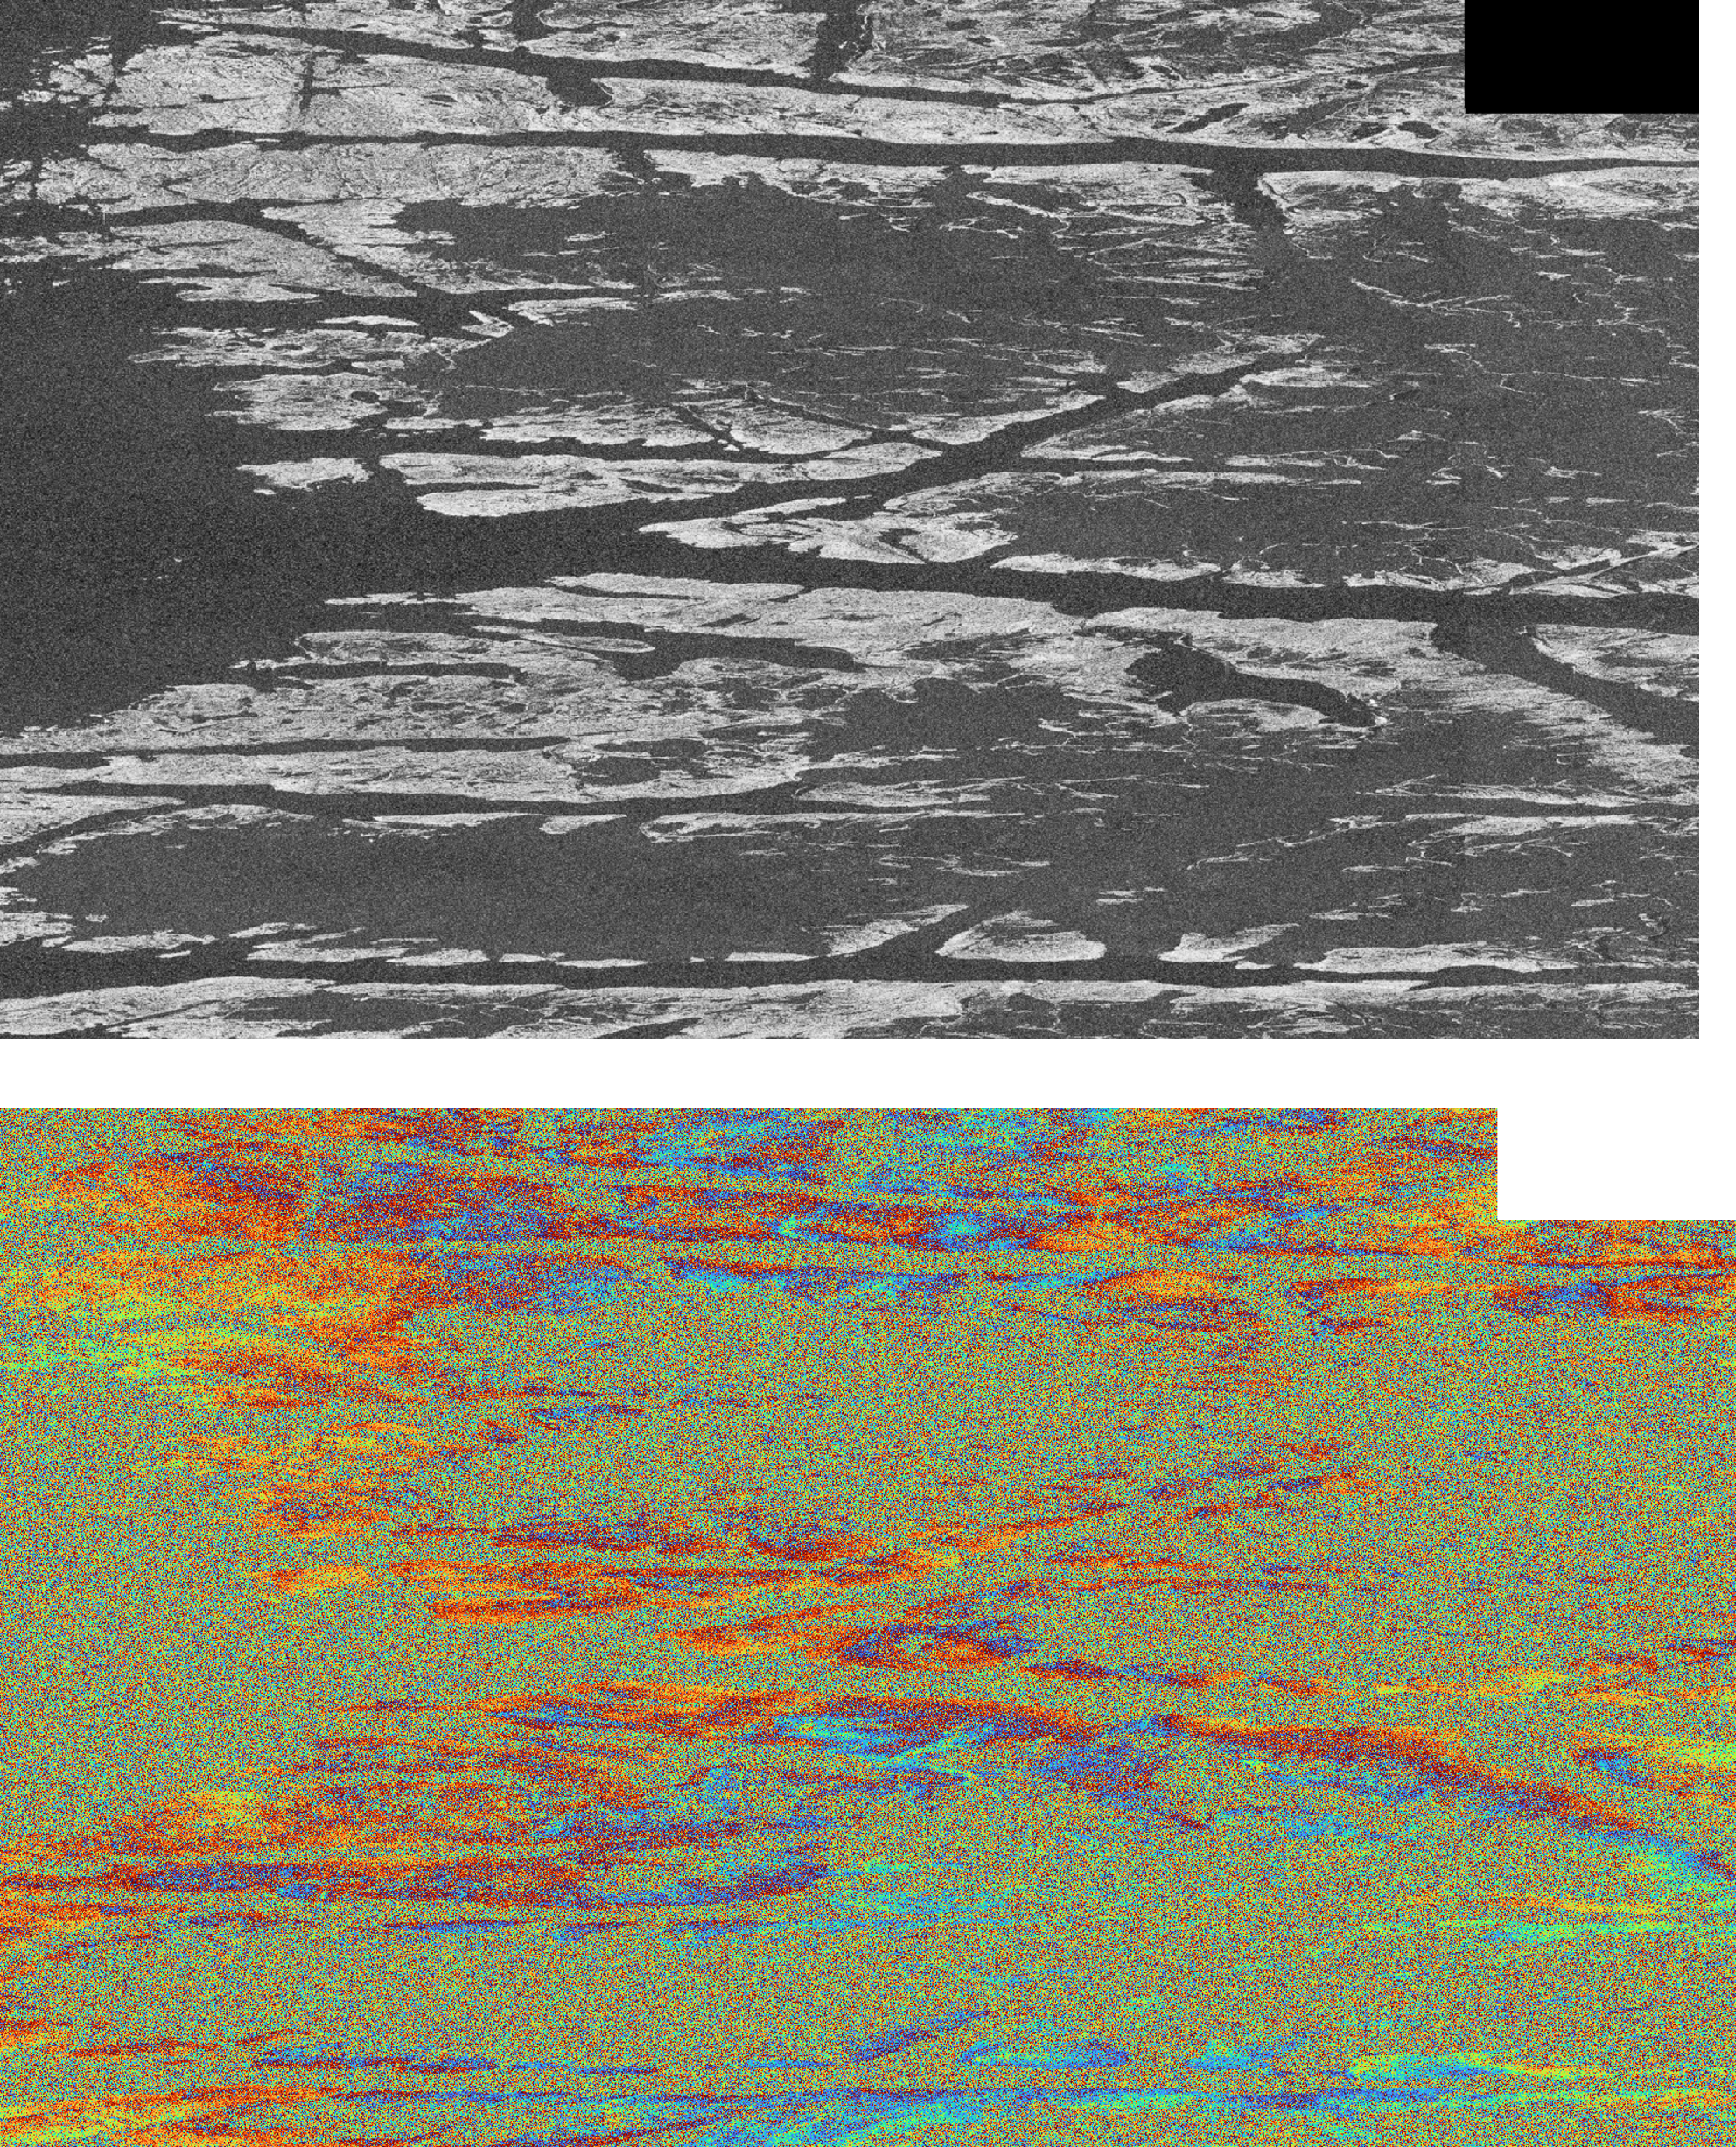
\includegraphics[width=0.9\textwidth]{Figures/strip_eq/cohe_phase_maps.png}
\caption{Interferometric coherence (top) and interferometric phase (bottom) maps derived from two \acs{stripeq} Sentinel-1 \acs{iw} products over Greenland. The input \acs{cslc} data were first co-registered using (\acs{esd}) and then independently mosaicked. The two maps exhibit seamless continuity across both burst and subswath boundaries. A slight increase in coherence in the second subswath is visible due to a higher oversampling factor, which enhances pixel-to-pixel correlation}
\label{fig:interf_coh_maps}
\end{figure}


These results confirm the validity of the \acs{stripeq} approach and its suitability for generating phase-consistent, analysis-ready \acs{sar} products from burst-mode acquisitions.

\subsection{Computational performance}
\label{sec:stripeq_computation}

The computational cost associated with the generation of a \acs{stripeq} product from a \acs{cslc} product is primarily driven by the need to meet the strict co-registration accuracy requirements outlined in the previous section. In particular, refining the azimuth alignment through Enhanced Spectral Diversity (\acs{esd}) constitutes the most computationally involved step. The overall processing workflow comprises the following main stages:

\begin{enumerate}
\item \textbf{Co-registration refinement via \acs{esd}.} For each pair of consecutive bursts within the same sub-swath, the \acs{esd} phase must be computed using only the overlap region. The \acs{esd} phase for each pixel in the overlap area is estimated as:
\begin{equation}
\phi_{ESD}^i(az, rg) = \arg\left((m_{i} \cdot s_{i}^{}) \cdot (m_{i+1} \cdot s_{i+1}^{})\right)
\label{eq:esd_phase}
\end{equation}
where $m_i$ and $s_i$ denote the master and slave complex samples, respectively, and $(i, i+1)$ refers to adjacent bursts. The coherence of the $i$-th burst is also calculated over the same overlap area and used as a weight in the estimation of $\phi_{ESD}^i$, which represents the ESD phase estimate for the $i$-th overlap region (i.e., the region shared by burst pair $(i, i+1)$).

\item \textbf{Phase-to-shift conversion.} All $\phi_{ESD}^i$ values computed in the previous step are aggregated across all burst pairs to estimate the residual azimuth shift. In the simplest case, this is done by averaging the phase values $\phi_{ESD}^i$, although more accurate estimation models can also be applied \citep{Martínez2016}. The computational cost of this step is minimal and can be considered negligible.

\item \textbf{Azimuth shift correction.} Each burst of the slave image is corrected in azimuth based on the estimated residual shift. Given that the residual azimuth error is typically close to a constant, this operation can be efficiently implemented using frequency-domain techniques (e.g., applying a phase ramp via FFT), resulting in low computational overhead compared to spatial-domain sinc-based interpolation. If this step cannot be implemented using a frequency-domain techniques, we need to consider for this step the same computational cost described in the \acs{cslc} product section. In particual, for every output pixel the interpolation algorithm evaluates a finite two-dimensional sinc kernel apodised by a Kaiser window.  
With an \(M\times N\) kernel the operation count is \(MN\) multiplications plus \(MN-1\) additions per pixel; high-fidelity implementations typically use a kernel of at least \(11\times11\). 

\item \textbf{Burst mosaicking.} The final step involves stitching the finely co-registered bursts together. This mosaicking operation is computationally inexpensive and primarily limited by I/O performance, as it entails reading, merging, and writing the corrected burst data.
\end{enumerate}

Overall, the dominant computational burden lies in the \acs{esd}-based refinement, particularly in calculating phase and coherence over multiple burst overlap regions. However, the subsequent steps are lightweight, and FFT-based implementations (when possible) help keep the overall processing pipeline efficient and scalable. 

It is worth noting that when the input \acs{cslc} data already meet the required co-registration accuracy—e.g., due to the use of a data-driven co-registration approach—the only step needed to generate the \acs{stripeq} product is the final mosaicking stage. In such cases, the additional computational cost is negligible.

\subsection{Criticalities and weakness}
\label{sec:stripeq_criticalities}


Two different scenarios must be considered regarding the generation of a \acs{stripeq} product from a \acs{cslc} input:

\begin{enumerate}
\item \textbf{Co-registration accuracy is already sufficient.} If the input \acs{cslc} already satisfies the co-registration accuracy requirements necessary for generating a valid \acs{stripeq} product---such as when a data-driven approach has been used during the co-registration process---and no co-registration refinement is required, no additional criticalities specific to the Stripmap-equivalent generation step are introduced. In this case, the process is limited to burst mosaicking, which is straightforward.

\item \textbf{Co-registration refinement is required.} If the input \acs{cslc} does not meet the required accuracy---e.g., in the case of Sentinel-1 data co-registered using only orbital information and a DEM---then the azimuth refinement described in the previous section must be applied. In this scenario, the generation of a \acs{stripeq} product inherits the same criticalities already discussed for the \acs{cslc} product, particularly the dependency on a consistently selected master image. This includes the need for robust master selection strategies and, in some cases, the updating of the reference master over time, both of which may introduce additional complexity into the processing workflow.
\end{enumerate}